\documentclass[11pt]{article}

% --- Packages ---
\usepackage[margin=0.9in]{geometry}
\usepackage{amsmath,amssymb,amsfonts}
\usepackage{graphicx}
\usepackage{tikz}
\usepackage{pgfplots}
\pgfplotsset{compat=1.18}
\usepackage{enumitem}
\usepackage{xcolor}
\usepackage{tcolorbox}
\usepackage{fancyhdr}
\usetikzlibrary{patterns}

% --- Header ---
\pagestyle{fancy}
\fancyhf{}
\lhead{\textbf{Algebra 2 \textbullet{} Lesson 4-3}}
\rhead{Multiplying \& Dividing Rational Expressions}
\cfoot{\thepage}

% --- DOK Tag Macro ---
\newcommand{\doktag}[1]{\hfill\textcolor{gray}{\small\textsf{[DOK #1]}}}

% --- Problem environment ---
\newtcolorbox{problem}[1]{
  colback=blue!3!white,
  colframe=blue!50!black,
  fonttitle=\bfseries,
  title={#1},
  breakable
}

% --- Workspace ---
\newcommand{\workspace}[1]{\vspace{#1}}

\title{\textbf{Lesson 4-3: Selected Problems} \\ \large Multiplying and Dividing Rational Expressions}
\author{}
\date{}

\begin{document}

\maketitle
\vspace{-2em}

% ====================================================================
% EXPLORE & REASON
% ====================================================================
\begin{problem}{Explore \& Reason \doktag{2}}
Consider the following graph of the function $y = x + 2$.

\begin{center}
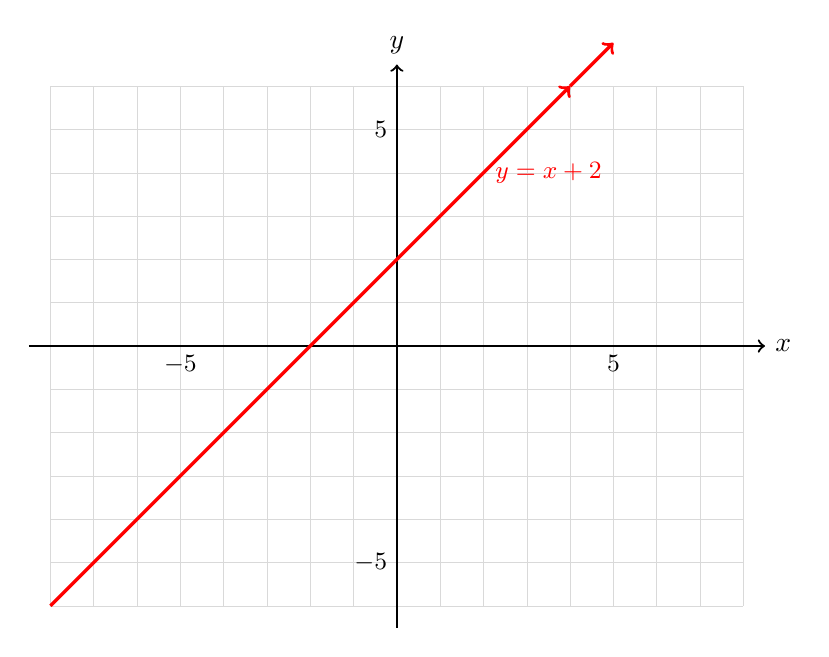
\begin{tikzpicture}[scale=0.55]
  % Grid
  \draw[very thin, gray!30] (-8,-6) grid (8,6);
  % Axes
  \draw[->, thick] (-8.5,0) -- (8.5,0) node[right] {$x$};
  \draw[->, thick] (0,-6.5) -- (0,6.5) node[above] {$y$};
  % Tick labels
  \foreach \x in {-5,5} \node[below] at (\x,0) {\small$\x$};
  \foreach \y in {-5,5} \node[left] at (0,\y) {\small$\y$};
  % Line y = x + 2
  \draw[red, very thick, ->] (-8,-6) -- (4,6);
  \draw[red, very thick, ->] (4,6) -- (5,7);
  \node[red] at (3.5,4) {\small$y=x+2$};
\end{tikzpicture}
\end{center}

\textbf{A.} What is the domain of this function?
\workspace{2.5cm}

\textbf{B.} Sketch a function that resembles the graph, but restrict its domain to exclude $2$.
\workspace{5cm}

\textbf{C.} \textbf{Use Structure} Consider the function you have sketched. What kind of function might have a graph like this? Explain.
\workspace{3cm}
\end{problem}

\newpage

% ====================================================================
% #13 HIGHER ORDER THINKING
% ====================================================================
\begin{problem}{\#13 --- Higher Order Thinking \doktag{3}}
Why are rational expressions closed under multiplication and division?
\workspace{8cm}
\end{problem}

\vspace{1em}

% ====================================================================
% #35 MAKE SENSE AND PERSEVERE
% ====================================================================
\begin{problem}{\#35 --- Make Sense and Persevere \doktag{2}}
An engineering firm wants to construct a cylindrical structure that will maximize the volume for a given surface area. Compare the ratios of the volume to surface area of each of the cylindrical structures shown, using the following formulas for volume and surface area of cylinders.
\[
V = \pi r^2 h \qquad SA = 2\pi r h + 2\pi r^2
\]

\begin{center}
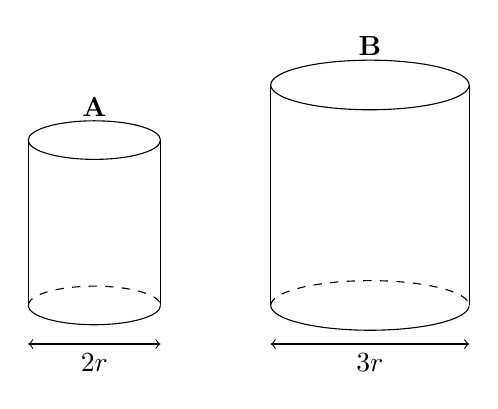
\begin{tikzpicture}[scale=0.7]
  % Cylinder A: radius 2r
  \begin{scope}[shift={(0,0)}]
    \draw (-1.2,0) -- (-1.2,3);
    \draw (1.2,0) -- (1.2,3);
    \draw (0,3) ellipse (1.2 and 0.35);
    \draw (-1.2,0) arc (180:360:1.2 and 0.35);
    \draw[dashed] (-1.2,0) arc (180:0:1.2 and 0.35);
    \draw[<->] (-1.2,-0.7) -- (1.2,-0.7) node[midway,below] {$2r$};
    \node at (0,3.6) {\textbf{A}};
  \end{scope}
  % Cylinder B: radius 3r, taller
  \begin{scope}[shift={(5,0)}]
    \draw (-1.8,0) -- (-1.8,4);
    \draw (1.8,0) -- (1.8,4);
    \draw (0,4) ellipse (1.8 and 0.45);
    \draw (-1.8,0) arc (180:360:1.8 and 0.45);
    \draw[dashed] (-1.8,0) arc (180:0:1.8 and 0.45);
    \draw[<->] (-1.8,-0.7) -- (1.8,-0.7) node[midway,below] {$3r$};
    \node at (0,4.7) {\textbf{B}};
  \end{scope}
\end{tikzpicture}
\end{center}

\textbf{a.} Calculate the ratio of volume to surface area for cylinder A.
\workspace{4cm}

\textbf{b.} Calculate the ratio of volume to surface area for cylinder B.
\workspace{4cm}

\textbf{c.} Which of these cylinders has a greater ratio of volume to surface area?
\workspace{2.5cm}
\end{problem}

\newpage

% ====================================================================
% #36 MODEL WITH MATHEMATICS
% ====================================================================
\begin{problem}{\#36 --- Model with Mathematics \doktag{2--3}}
Lupe designed a carnival game that involves tossing a beanbag into the box shown. In order to win a prize, the beanbag must fall inside the black rectangle. The probability of winning is equal to the ratio of the area of the black rectangle to the total area of the face of the box shown. Find the ratio that represents this probability in simplified form.

\begin{center}
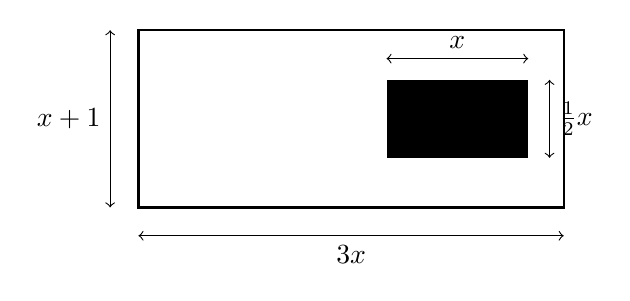
\begin{tikzpicture}[scale=0.9]
  % Outer rectangle: width 3x, height x+1
  \draw[thick] (0,0) rectangle (6,2.5);
  % Inner black rectangle: width x, height (1/2)x
  \fill[black] (3.5,0.7) rectangle (5.5,1.8);
  % Dimension labels for outer
  \draw[<->] (0,-0.4) -- (6,-0.4) node[midway,below] {$3x$};
  \draw[<->] (-0.4,0) -- (-0.4,2.5) node[midway,left] {$x+1$};
  % Dimension labels for inner
  \draw[<->] (3.5,2.1) -- (5.5,2.1) node[midway,above] {$x$};
  \draw[<->] (5.8,0.7) -- (5.8,1.8) node[midway,right] {$\tfrac{1}{2}x$};
\end{tikzpicture}
\end{center}

\workspace{8cm}
\end{problem}

\newpage

% ====================================================================
% #40 PERFORMANCE TASK
% ====================================================================
\begin{problem}{\#40 --- Performance Task \doktag{2}}
The approximate annual interest rate $r$ of a monthly installment loan is given by the formula:
\[
r = \dfrac{\left[\dfrac{24(nm - p)}{n}\right]}{\left(p + \dfrac{nm}{12}\right)}
\]
where $n$ is the total number of payments, $m$ is the monthly payment, and $p$ is the amount financed.

\vspace{0.5em}
\textbf{Part A.} Find the approximate annual interest rate (to the nearest percent) for a \textbf{four-year signature loan of \$20{,}000} that has monthly payments of \$500.
\workspace{6cm}

\textbf{Part B.} Find the approximate annual interest rate (to the nearest tenth percent) for a \textbf{five-year auto loan of \$40{,}000} that has monthly payments of \$750.
\workspace{6cm}
\end{problem}

\end{document}
